\documentclass[12pt,a4paper]{article}

% ---- Packages ----
\usepackage[utf8]{inputenc}
\usepackage[T1]{fontenc}
\usepackage{times}
\usepackage{geometry}
\geometry{left=2.5cm, right=2.5cm, top=2.5cm, bottom=2.5cm}
\usepackage{amsmath,amssymb}
\usepackage{graphicx}
\usepackage{booktabs}
\usepackage{caption}
\usepackage{hyperref}
\hypersetup{colorlinks=true, linkcolor=black, citecolor=black, urlcolor=blue}
\usepackage{natbib}
\bibliographystyle{unsrt}
\usepackage{setspace}
\onehalfspacing
\usepackage{indentfirst}
\setlength{\parindent}{1.5em}
\usepackage{array}
\usepackage{multirow}
\usepackage{tabto}

\renewcommand{\abstractname}{Abstrak}

% ---- Title (Indonesia) ----
\title{\Large\textbf{Evaluasi Komparatif Teknik Penskalaan Fitur\\
       pada Berbagai Klasifikator dan Domain}}

\author{
  Amri Reza Wahyudin$^{1*}$, Sri Murdiawati$^{2}$, Juan Adi Putra$^{3}$, Erliyan Redy Susanto$^{4}$ \\[4pt]
  \normalsize
  $^{1,2,3,4}$Magister Ilmu Komputer, Fakultas Teknik dan Ilmu Komputer,\\
  \normalsize
  Universitas Teknokrat Indonesia \\[4pt]
  \normalsize
  $^{*}$\textit{Penulis korespondensi:} \texttt{amri\_reza\_wahyudin@teknokrat.ac.id}
}
\date{}

\begin{document}
\hbadness=10000
\hfuzz=30pt
\emergencystretch=3em

\maketitle
\footnotetext{Kode dan data: \url{https://github.com/AmZaDin14/feature-scaling-study}}

% ============================================================
\begin{abstract}
\noindent
Penskalaan fitur sangat krusial pada algoritma \textit{machine learning} berbasis jarak, namun teknik optimal pada berbagai klasifikator, domain, dan tipe permasalahan belum diketahui secara pasti. Studi ini mengevaluasi enam konfigurasi penskalaan---Normalisasi \textit{Min-Max}, Standardisasi \textit{Z-Score}, \textit{Robust Scaling} (IQR), \textit{MaxAbs Scaling}, dan \textit{Quantile Transformation}---dibandingkan dengan \textit{baseline} data mentah pada enam \textit{dataset} standar dan tujuh klasifikator (\textit{k-NN} dengan jarak Euclidean, Manhattan, dan Cosine; \textit{SVM} dengan kernel Linear dan RBF; \textit{Decision Tree}; dan \textit{Random Forest}), termasuk empat \textit{dataset} multikelas (3--10 kelas). Sebanyak 3.384 konfigurasi dievaluasi menggunakan validasi silang bertingkat 5-lipat. Standardisasi \textit{Z-Score} menempati peringkat pertama (0,8561), diikuti \textit{Min-Max} (0,8530, $p=0,123$---setara secara statistik) dan \textit{MaxAbs} (0,8506). Pemilihan \textit{scaler} optimal bergantung pada domain: \textit{Z-Score} unggul pada data medis dan biologis multikelas, \textit{Min-Max} pada ruang fitur terbatas, \textit{MaxAbs} pada data berdimensi tinggi, dan data mentah memadai ketika fitur telah berskala alami. Klasifikator berbasis jarak meningkat 4,5--7,7\% dengan penskalaan, sementara model berbasis pohon hampir invarian ($<$0,2\%). Hasil ini memberikan acuan praktis bagi pengambilan keputusan prapemrosesan dalam tugas klasifikasi. Kode sumber dan implementasi lengkap eksperimen ini tersedia secara terbuka pada repositori \url{https://github.com/AmZaDin14/feature-scaling-study}.

\vspace{6pt}
\noindent\textbf{Kata kunci:} penskalaan fitur, normalisasi, standardisasi, \textit{robust scaling}, \textit{MaxAbs}, \textit{QuantileTransformer},
\textit{k-nearest neighbors}, \textit{SVM}, klasifikasi multikelas, studi komparatif
\end{abstract}

% ============================================================
\section{Pendahuluan}
\label{sec:intro}

Algoritma \textit{k-Nearest Neighbors} (k-NN) banyak digunakan dalam tugas
klasifikasi \cite{cunningham2021knn,halder2024knn}, yang beroperasi berdasarkan
prinsip kedekatan dalam ruang multidimensi \cite{bakri2025knn,sultana2022knn}.
Akan tetapi, efektivitas \textit{k-NN}---dan seluruh klasifikator berbasis
jarak---sangat bergantung pada skala fitur. Pada \textit{dataset} empiris,
fitur-fitur seringkali memiliki satuan dan rentang nilai yang sangat berbeda,
seperti usia (0--100) dibandingkan penghasilan ($0$--$10^6$). Hal ini menimbulkan
masalah fundamental: fitur dengan magnitudo lebih besar secara matematis akan
mendominasi perhitungan jarak tanpa memandang signifikansi prediktifnya
\cite{mutoffar2025ml,cetin2024distance,pagan2023scaling}.

\textit{Support Vector Machines} (SVM) juga sensitif terhadap skala fitur
\cite{guido2024svm,pinheiro2025scaling}. Regularisasi memberikan penalti secara
seragam pada koefisien, sehingga fitur tak terskala dengan rentang lebih besar
menerima bobot yang lebih kecil secara tidak proporsional. Model berbasis pohon
(\textit{Decision Tree}, \textit{Random Forest}) secara teoretis bersifat
invarian terhadap penskalaan \cite{ahsan2021scaling}, karena pohon keputusan
melakukan pemisahan berdasarkan ambang batas per fitur secara independen.

Meskipun pentingnya penskalaan fitur telah diketahui secara luas, literatur
ilmiah masih kekurangan tolok ukur komprehensif yang secara simultan
membandingkan beberapa teknik penskalaan pada beberapa famili klasifikator, baik
pada permasalahan biner maupun multikelas. Studi yang ada cenderung membatasi
perbandingan pada \textit{Min-Max} versus \textit{Z-Score} pada satu algoritma
\cite{henderi2021minmax,manurung2025knn}, atau mengevaluasi satu teknik pada
beberapa algoritma \cite{pagan2023scaling}. Belum ada studi sebelumnya yang
secara sistematis membandingkan enam teknik penskalaan---termasuk \textit{MaxAbs
Scaling} dan \textit{Quantile Transformation}---pada tujuh klasifikator di
\textit{dataset} biner dan multikelas dengan validasi statistik.

Studi ini menjawab celah-celah tersebut melalui tiga pertanyaan penelitian:

\begin{enumerate}
  \item[\textbf{RQ1:}] Teknik penskalaan manakah yang menghasilkan kinerja
  klasifikasi keseluruhan terbaik pada pengaturan biner maupun multikelas?
  \item[\textbf{RQ2:}] Apakah teknik penskalaan optimal bergantung pada jenis
  klasifikator yang digunakan?
  \item[\textbf{RQ3:}] Apakah teknik penskalaan optimal bergantung pada domain
  data dan tipe permasalahan (biner vs. multikelas)?
\end{enumerate}

Kami juga memperkenalkan \textit{MaxAbs Scaling} dan \textit{Quantile
Transformation}---teknik yang tersedia di pustaka standar namun jarang
diukurbandingkan terhadap \textit{Min-Max}, \textit{Z-Score}, dan
\textit{Robust Scaling} dalam kerangka komparatif terpadu.

% ============================================================
\section{Penelitian Terkait}
\label{sec:related}

\subsection{Dasar-Dasar Penskalaan Fitur}
\label{sec:fundamentals}

Penskalaan fitur mentransformasikan rentang numerik fitur ke suatu skala yang
seragam. Lima pendekatan utama dievaluasi dalam studi ini, yang didefinisikan
oleh Persamaan~\eqref{eq:euclidean} hingga \eqref{eq:quantile}.

Jarak Euclidean merupakan metrik yang mendasari sebagian besar klasifikator
berbasis jarak. Diberikan dua titik data $\mathbf{x}$ dan $\mathbf{y}$ dalam
ruang $n$-dimensi, jaraknya adalah:
\begin{equation}
  d(\mathbf{x}, \mathbf{y}) = \sqrt{\sum_{i=1}^{n} (x_i - y_i)^2}
  \label{eq:euclidean}
\end{equation}
Tanpa penskalaan fitur, fitur dengan magnitudo lebih besar mendominasi
penjumlahan ini secara tidak proporsional.

\textbf{Normalisasi \textit{Min-Max}} menskala ulang fitur secara linear ke
rentang tetap, umumnya $[0, 1]$:
\begin{equation}
  x_{\text{norm}} = \frac{x - x_{\min}}{x_{\max} - x_{\min}}
  \label{eq:minmax}
\end{equation}
Metode ini mempertahankan bentuk distribusi asli namun sensitif terhadap pencilan
(\textit{outliers}), karena nilai ekstrem akan memampatkan data lainnya ke dalam
sub-rentang yang sempit.

\textbf{Standardisasi \textit{Z-Score}} memusatkan fitur ke rataan nol dan
varians satuan:
\begin{equation}
  x_{\text{std}} = \frac{x - \mu}{\sigma}
  \label{eq:zscore}
\end{equation}
Berbeda dengan \textit{Min-Max}, \textit{Z-Score} tidak membatasi nilai ke
rentang tetap, sehingga lebih kokoh terhadap pencilan sambil mempertahankan
informasi jarak relatif.

\textbf{\textit{Robust Scaling}} menggunakan median dan rentang interkuartil
(IQR):
\begin{equation}
  x_{\text{robust}} = \frac{x - \text{median}(x)}{\text{IQR}(x)}
  \label{eq:robust}
\end{equation}
Dengan menggunakan statistik yang kokoh, metode ini menjadi yang paling tangguh
terhadap pencilan \cite{templ2023robust}.

\textbf{\textit{MaxAbs Scaling}} menskala setiap fitur berdasarkan nilai absolut
maksimumnya, memetakan ke rentang $[-1, 1]$:
\begin{equation}
  x_{\text{maxabs}} = \frac{x}{\max(|x|)}
  \label{eq:maxabs}
\end{equation}
Metode ini mempertahankan \textit{sparsity} (nilai nol tetap nol) dan umum
digunakan untuk data jarang (\textit{sparse data}).

\textbf{\textit{Quantile Transformation}} memetakan setiap fitur ke distribusi
seragam atau normal melalui invers fungsi distribusi kumulatif empiris:
\begin{equation}
  x_{\text{quantile}} = F^{-1}_{\text{uniform}}(F_{\text{empirical}}(x))
  \label{eq:quantile}
\end{equation}
Berbeda dengan metode linear di atas, \textit{Quantile Transformation} bersifat
non-linear dan dapat menangani distribusi arbitrer
\cite{demircioglu2024normalization}.

Tabel~\ref{tbl:scalers} merangkum keenam teknik tersebut.

\begin{table}[ht]
\centering
\caption{Ringkasan teknik penskalaan fitur.}
\label{tbl:scalers}
\begin{tabular}{lccc}
\toprule
Teknik & Formula & Rentang & Linearitas \\
\midrule
Min-Max         & Pers.~\eqref{eq:minmax}  & $[0, 1]$     & Linear \\
Z-Score         & Pers.~\eqref{eq:zscore}  & Tak terbatas  & Linear \\
Robust          & Pers.~\eqref{eq:robust}  & Tak terbatas  & Linear \\
MaxAbs          & Pers.~\eqref{eq:maxabs}  & $[-1, 1]$    & Linear \\
Quantile        & Pers.~\eqref{eq:quantile}& $(0, 1)$     & Non-linear \\
\bottomrule
\end{tabular}
\end{table}

\subsection{Studi Komparatif Sebelumnya}
\label{sec:prev}

Pagan dkk.~\cite{pagan2023scaling} meneliti \textit{Min-Max}, \textit{Z-Score},
dan \textit{decimal scaling} pada \textit{k-NN} di sepuluh \textit{dataset},
dan menemukan bahwa pemilihan teknik penskalaan secara signifikan memengaruhi
kinerja namun bervariasi antar \textit{dataset}. Henderi
dkk.~\cite{henderi2021minmax} membandingkan \textit{Min-Max} dan \textit{Z-Score}
pada \textit{k-NN} untuk klasifikasi kanker payudara, melaporkan keunggulan
\textit{Min-Max} (98\% vs 97\%). Firmansyah dan Astuti~\cite{firmansyah2024stroke}
membandingkan standardisasi dan normalisasi pada \textit{k-NN} untuk klasifikasi
stroke. Pinheiro dkk.~\cite{pinheiro2025scaling} baru-baru ini melakukan studi
skala besar terhadap 12 \textit{scaler} pada 14 algoritma di 16 \textit{dataset},
yang menunjukkan bahwa metode ensemble kokoh terhadap penskalaan sementara SVM
sangat sensitif.

Akan tetapi, studi-studi ini memiliki keterbatasan yang serupa: perbandingan
terbatas pada satu klasifikator (\textit{k-NN}), jarang menyertakan
\textit{MaxAbs} atau \textit{Quantile Scaling}, dan seringkali tidak menyertakan
evaluasi multikelas. Studi kami menjawab keterbatasan ini dengan memperluas
perbandingan ke tujuh klasifikator, enam \textit{scaler} (termasuk
\textit{MaxAbs} dan \textit{Quantile}), dan enam \textit{dataset} yang mencakup
permasalahan biner maupun multikelas, dengan validasi statistik melalui uji
peringkat-bertanda \textit{Wilcoxon} berpasangan.

% ============================================================
\section{Metodologi}
\label{sec:method}

\subsection{Dataset}
\label{sec:datasets}

Enam \textit{dataset} klasifikasi standar dipilih untuk merepresentasikan
beragam domain dan tipe permasalahan. Tabel~\ref{tbl:datasets} merangkum
karakteristiknya. Empat dari enam \textit{dataset} bersifat multikelas
(3--10 kelas), memungkinkan evaluasi efek penskalaan di luar pengaturan biner.

\begin{table}[ht]
\centering
\caption{Karakteristik \textit{dataset}.}
\label{tbl:datasets}
\begin{tabular}{lcrrl}
\toprule
Dataset & Domain & Sampel & Fitur & Kelas \\
\midrule
Pima Indians Diabetes  & Medis      & 768  &  8 & 2 \\
Breast Cancer Wisconsin & Medis     & 569  & 30 & 2 \\
Wine                   & Kimia      & 178  & 13 & 3 \\
Digits                 & Citra      & 1.797& 64 & 10 \\
Yeast                  & Biologi    & 1.484&  8 & 10 \\
Segment                & Segmentasi & 2.310& 19 & 7 \\
\bottomrule
\end{tabular}
\end{table}

Pima Indians Diabetes mengandung nilai nol yang tidak valid secara biologis
pada fitur seperti Glukosa dan BMI, yang diimputasi menggunakan median
(sejalan dengan~\cite{pristyanto2022diabetes}). Semua \textit{dataset} lainnya
digunakan dalam bentuk aslinya---Wine dan Digits sebagai permasalahan multikelas
(masing-masing 3 dan 10 kelas), serta Yeast dan Segment sebagaimana publikasi aslinya.

\subsection{Teknik Penskalaan}
\label{sec:scalers}

Enam konfigurasi penskalaan dievaluasi, sebagaimana dirangkum dalam
Tabel~\ref{tbl:scaler-config}. Seluruh \textit{scaler} diimplementasikan melalui
\texttt{scikit-learn} dengan parameter bawaan.

\begin{table}[ht]
\centering
\caption{Konfigurasi penskalaan yang dievaluasi.}
\label{tbl:scaler-config}
\begin{tabular}{llll}
\toprule
Scaler & Tipe & Rentang & Sifat Utama \\
\midrule
None (Mentah) & Tanpa transformasi & Asli & Baseline \\
Min-Max    & Pers.~\eqref{eq:minmax} & $[0, 1]$    & Mempertahankan distribusi \\
Z-Score    & Pers.~\eqref{eq:zscore} & Tak terbatas & Memusatkan data \\
Robust     & Pers.~\eqref{eq:robust} & Tak terbatas & Berbasis Median/IQR \\
MaxAbs     & Pers.~\eqref{eq:maxabs} & $[-1, 1]$   & Mempertahankan \textit{sparsity} \\
Quantile   & Pers.~\eqref{eq:quantile} & $(0, 1)$ & Non-linear \\
\bottomrule
\end{tabular}
\end{table}

\subsection{Klasifikator}
\label{sec:classifiers}

Tujuh klasifikator dievaluasi, sebagaimana ditunjukkan pada
Tabel~\ref{tbl:classifiers}. Untuk varian \textit{k-NN}, seluruh nilai $k$ dari
1 hingga 30 diuji untuk menangkap sensitivitas terhadap ukuran tetangga.
Klasifikator non-\textit{k-NN} menggunakan parameter bawaan \texttt{scikit-learn}.

\begin{table}[ht]
\centering
\caption{Konfigurasi klasifikator.}
\label{tbl:classifiers}
\begin{tabular}{cll}
\toprule
No. & Klasifikator & Parameter \\
\midrule
1 & k-NN (Euclidean) & $k = 1,\dots,30$, metrik = Euclidean \\
2 & k-NN (Manhattan) & $k = 1,\dots,30$, metrik = Manhattan \\
3 & k-NN (Cosine)    & $k = 1,\dots,30$, metrik = Cosine \\
4 & SVM (Linear)     & \textit{kernel} = linear \\
5 & SVM (RBF)        & \textit{kernel} = rbf \\
6 & Decision Tree    & CART, bawaan \\
7 & Random Forest    & 100 \textit{estimator}, bawaan \\
\bottomrule
\end{tabular}
\end{table}

\subsection{Protokol Eksperimental}
\label{sec:protocol}

Setiap \textit{dataset} diproses sebagai berikut:
\begin{enumerate}
  \item \textbf{Prapemrosesan:} Nilai nol tidak valid diimputasi dengan median
  (khusus Pima).
  \item \textbf{Validasi silang:} Pembagian bertingkat 5-lipat yang
  mempertahankan distribusi kelas \cite{bates2023crossval}.
  \item \textbf{Penskalaan:} Setiap \textit{scaler} dipasangkan pada lipatan
  pelatihan, lalu diterapkan pada lipatan pelatihan dan validasi secara
  independen---memastikan tidak terjadi kebocoran data.
  \item \textbf{Evaluasi:} Klasifikator dilatih pada lipatan pelatihan yang
  telah diskala, lalu dievaluasi pada lipatan validasi yang telah diskala.
  \item \textbf{Metrik:} Akurasi (rata-rata $\pm$ simpangan baku antar lipatan),
  presisi, \textit{recall}, \textit{F1-score}, AUC, spesifisitas, sensitivitas.
\end{enumerate}

Untuk evaluasi multikelas, presisi, \textit{recall}, dan \textit{F1-score}
dihitung dengan rata-rata terbobot (\textit{weighted averaging}) untuk
memperhitungkan ketidakseimbangan kelas. AUC dihitung menggunakan skema
satu-lawan-sisanya (\textit{one-vs-rest}, OvR). Sensitivitas dan spesifisitas
dirata-ratakan secara makro di seluruh kelas, memberikan bobot yang sama pada
setiap kelas tanpa memandang prevalensinya.

Pemilihan $k=1,\dots,30$ untuk \textit{k-NN} mencakup rentang praktis penuh
dari batas keputusan yang sangat lokal ($k=1$) hingga hampir global ($k=30$),
menangkap rezim \textit{overfitting} maupun \textit{underfitting}. Klasifikator
non-\textit{k-NN} menggunakan hiperparameter bawaan \texttt{scikit-learn}:
SVM dengan $C=1$ dan RBF $\gamma=1/n_{\text{fitur}}$, \textit{Decision Tree}
dengan kedalaman tak terbatas dan \textit{Gini impurity}, serta \textit{Random
Forest} dengan 100 pohon. Nilai-nilai bawaan ini merupakan \textit{baseline}
yang mapan dalam studi ML komparatif dan menghindari pencampuran efek
penskalaan dengan artefak penalaan hiperparameter, yang ditunda untuk
penelitian selanjutnya.

Pemilihan validasi silang bertingkat 5-lipat menyeimbangkan bias dan varians
sambil memastikan setiap lipatan mempertahankan proporsi kelas asli. Lima
lipatan memberikan timbang terima yang baik antara varians tinggi dari validasi
silang 2-lipat dan biaya komputasi tinggi dari validasi silang 10-lipat, dan
pengambilan sampel bertingkat mencegah bias optimistis pada kelas minoritas,
yang sangat krusial untuk \textit{dataset} multikelas dengan distribusi tidak
seimbang (misalnya, Yeast dengan 10 kelas).

Secara total: 6 \textit{dataset} $\times$ 6 \textit{scaler} $\times$
(3 varian \textit{k-NN} $\times$ 30 nilai $k$ + 4 klasifikator non-\textit{k-NN})
= \textbf{3.384 konfigurasi}, masing-masing dievaluasi dengan validasi silang
bertingkat 5-lipat (\textbf{16.920 total pemasangan model}).

\subsection{Analisis Statistik}
\label{sec:stats}

Uji peringkat-bertanda \textit{Wilcoxon} berpasangan
\cite{amorim2023scaling} dilakukan untuk setiap pasangan \textit{scaler} pada
seluruh konfigurasi yang berpadanan (\textit{dataset}, klasifikator, nilai $k$).
Uji non-parametrik ini dipilih karena perbedaan kinerja antar \textit{scaler}
tidak dijamin mengikuti distribusi normal. Signifikansi dinilai pada
$\alpha = 0,05$.

% ============================================================
\section{Hasil}
\label{sec:results}

\subsection{RQ1: Kinerja Penskalaan Keseluruhan}
\label{sec:rq1}

Teknik penskalaan manakah yang memberikan akurasi terbaik di seluruh kondisi?
Dirata-ratakan pada seluruh \textit{dataset} dan klasifikator, keenam teknik
penskalaan menunjukkan peringkat seperti pada Tabel~\ref{tbl:ranking}.

\begin{table}[ht]
\centering
\caption{Peringkat \textit{scaler} keseluruhan berdasarkan rata-rata akurasi
pada validasi silang bertingkat 5-lipat.}
\label{tbl:ranking}
\begin{tabular}{lcc}
\toprule
Scaler & Rata-rata Akurasi & Simpangan Baku \\
\midrule
\textbf{Z-Score} & \textbf{0,8561} & 0,147 \\
Min-Max          & 0,8530 & 0,150 \\
MaxAbs           & 0,8506 & 0,151 \\
Robust           & 0,8370 & 0,146 \\
Quantile         & 0,8345 & 0,156 \\
Mentah (Raw)     & 0,8050 & 0,146 \\
\bottomrule
\end{tabular}
\end{table}

Pada tingkat agregat, jawaban untuk RQ1 adalah: \textbf{\textit{Z-Score}
menempati peringkat pertama, namun tiga \textit{scaler} teratas
(\textit{Z-Score}, \textit{Min-Max}, \textit{MaxAbs}) berada dalam kelompok
yang berdekatan.} Uji peringkat-bertanda \textit{Wilcoxon} menunjukkan:

\begin{itemize}
  \item \textbf{\textit{Z-Score} vs \textit{Min-Max}:} $p = 0,123$
  (tidak signifikan; secara statistik setara)
  \item \textbf{\textit{Z-Score} vs \textit{MaxAbs}:} $p = 0,002$
  (signifikan, namun efek kecil: +0,0055)
  \item \textbf{\textit{Z-Score} vs Mentah:} $p < 0,001$ (signifikan)
  \item \textbf{\textit{Min-Max} vs \textit{MaxAbs}:} $p < 0,001$
  (signifikan, +0,0024)
  \item \textbf{Semua \textit{scaler} vs Mentah:} $p < 0,01$ (semua signifikan)
\end{itemize}

Hasil agregat ini mengonfirmasi bahwa \textbf{penskalaan apa pun secara
signifikan lebih baik daripada tanpa penskalaan.} Namun, selisih sempit antar
pesaing teratas (hanya 0,0055 antara \textit{Z-Score} dan \textit{MaxAbs})
menegaskan bahwa pertanyaan praktisnya bukanlah \emph{\textit{scaler} mana yang
menang secara keseluruhan} melainkan \emph{\textit{scaler} mana yang terbaik
untuk data spesifik saya}.

\subsection{RQ2: Pengaruh Jenis Klasifikator}
\label{sec:rq2}

Apakah teknik penskalaan optimal bergantung pada klasifikator yang digunakan?
Gambar~\ref{fig:heatmap} dan Tabel~\ref{tbl:classifier-sensitivity} menjawab
pertanyaan ini.

\begin{figure}[ht]
\centering
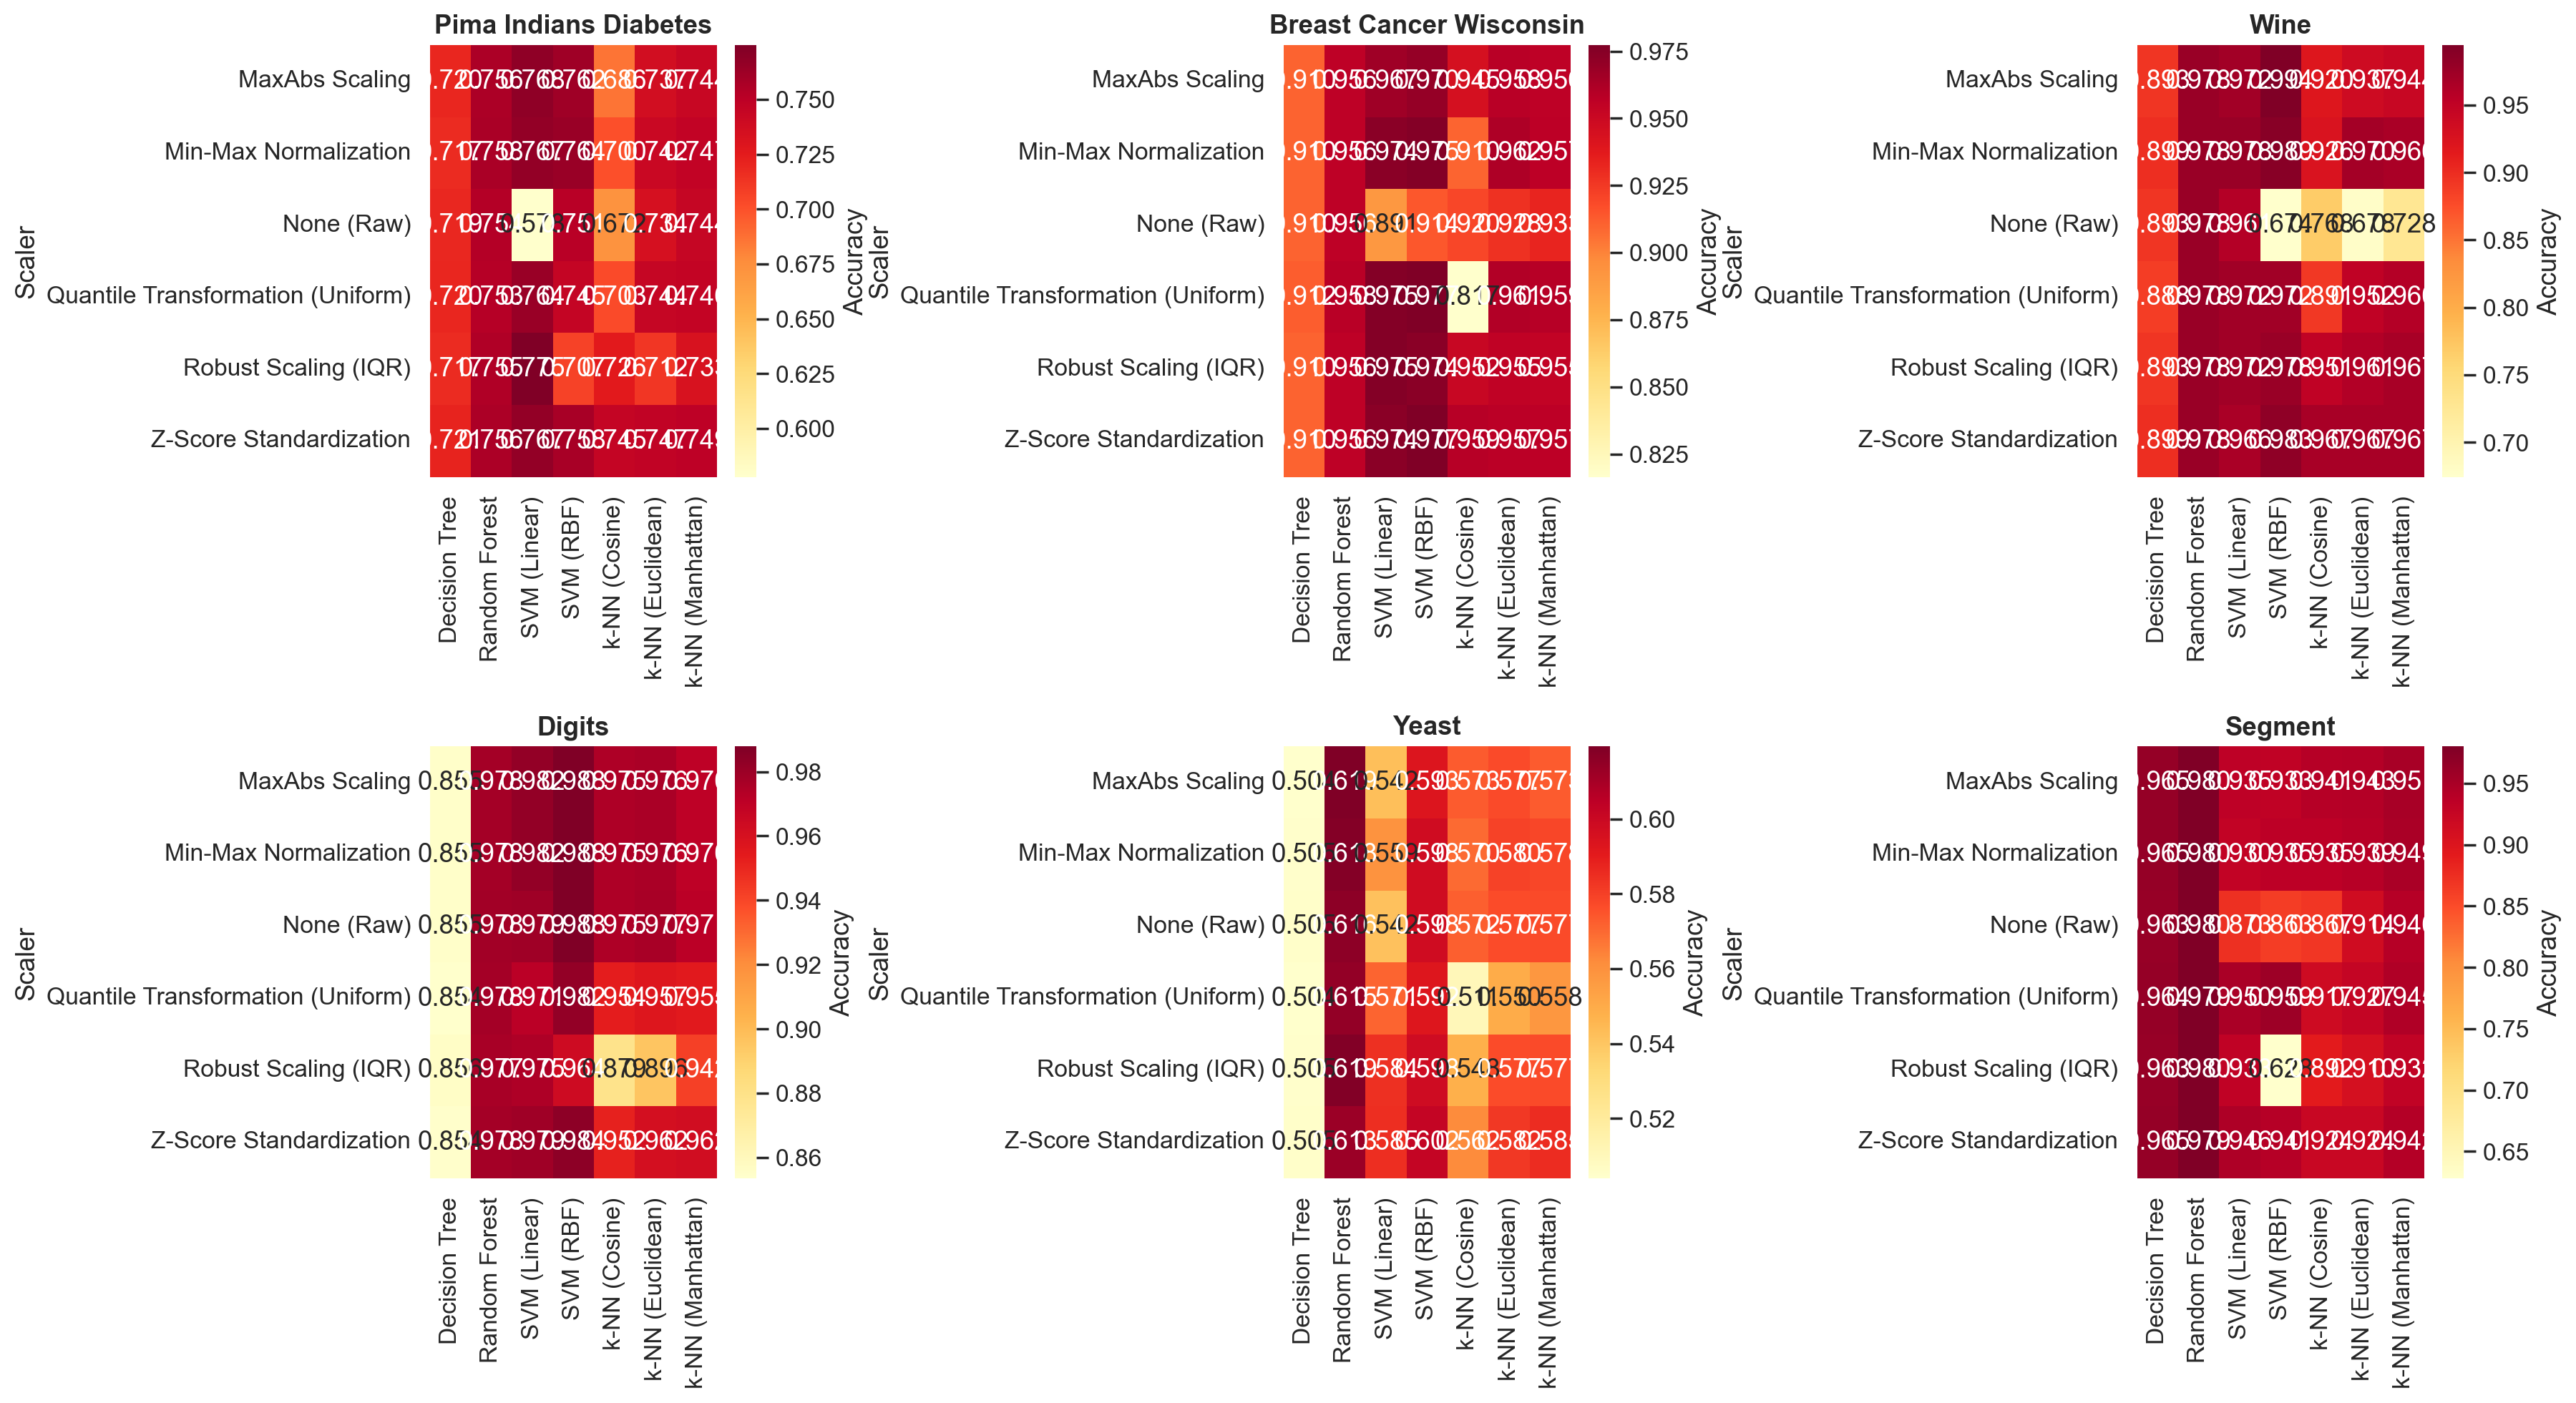
\includegraphics[width=\textwidth]{figures/accuracy_heatmap.png}
\caption{Peta panas akurasi yang menunjukkan rata-rata akurasi setiap
kombinasi \textit{scaler}--klasifikator per \textit{dataset}. Sel yang lebih
gelap menunjukkan akurasi lebih tinggi.}
\label{fig:heatmap}
\end{figure}

\begin{table}[ht]
\centering
\caption{Dampak penskalaan berdasarkan jenis klasifikator (rata-rata akurasi
pada seluruh \textit{dataset}).}
\label{tbl:classifier-sensitivity}
\begin{tabular}{lccc}
\toprule
Klasifikator & Scaler Terbaik & Akurasi Terbaik & Peningkatan \\
\midrule
k-NN (Euclidean) & Min-Max   & 0,8615 & +0,0602 \\
k-NN (Manhattan) & Min-Max   & 0,8612 & +0,0456 \\
k-NN (Cosine)    & Z-Score   & 0,8514 & +0,0556 \\
SVM (Linear)     & Z-Score   & 0,8696 & +0,0656 \\
SVM (RBF)        & Min-Max   & 0,8749 & +0,0769 \\
Decision Tree    & Z-Score   & 0,8091 & +0,0015 \\
Random Forest    & MaxAbs    & 0,8779 & +0,0010 \\
\bottomrule
\end{tabular}
\end{table}

Tiga pola berbeda muncul:

\textbf{Klasifikator berbasis jarak (\textit{k-NN}, SVM) sangat bergantung pada
penskalaan.} Tanpa penskalaan, rata-rata akurasi \textit{k-NN} turun sebesar
4,6--6,0 poin persentase. SVM dengan kernel linear bahkan lebih sensitif
(penurunan 6,6 pp dengan data mentah). SVM dengan kernel RBF menunjukkan
peningkatan terbesar dari penskalaan (+7,7 pp), mengindikasikan bahwa batas
keputusan lokal kernel RBF memperoleh manfaat substansial dari penskalaan
fitur yang tepat.

Di antara varian \textit{k-NN}, \textit{MaxAbs} dan \textit{Z-Score} menghasilkan
akurasi paling stabil pada seluruh nilai $k$ (Gambar~\ref{fig:knn-stability}).
\textit{Min-Max} menunjukkan fluktuasi tajam pada data Pima Diabetes akibat
pemampatan pencilan.

\begin{figure}[ht]
\centering
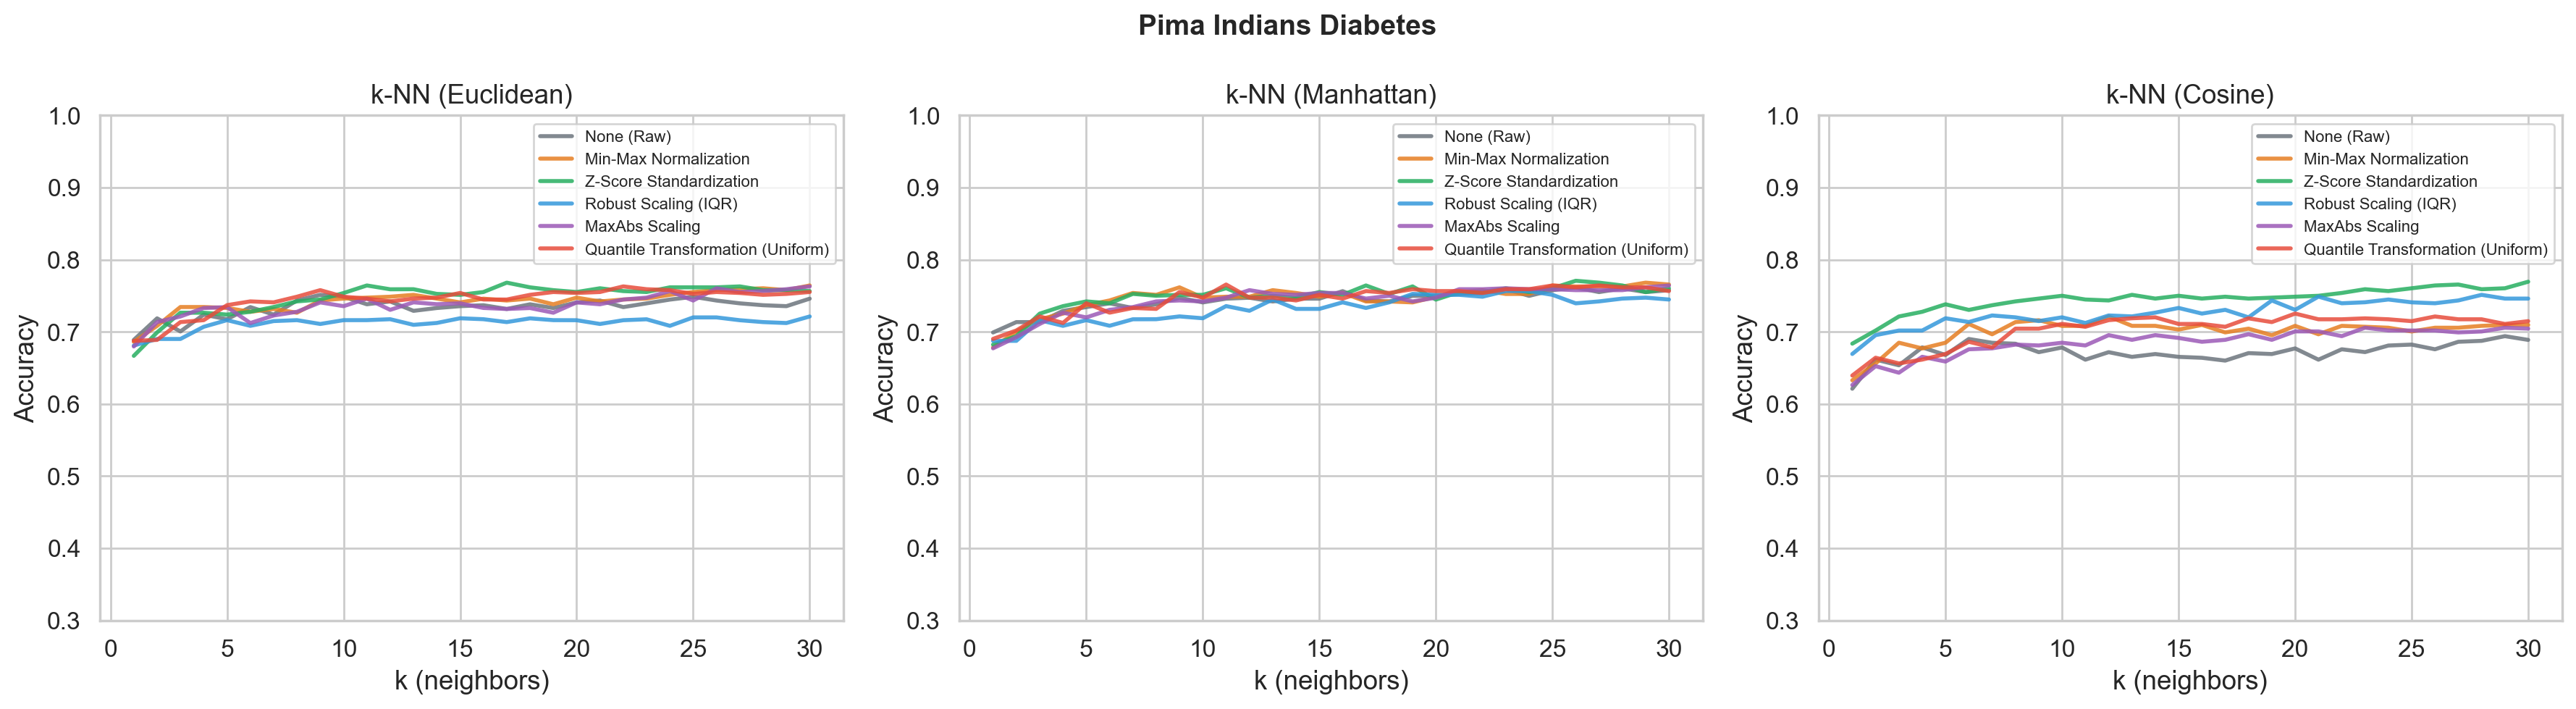
\includegraphics[width=0.75\textwidth]{figures/knn_stability_pima_indians_diabetes.png}
\caption{Akurasi \textit{k-NN} (Euclidean) versus $k$ pada Pima Indians Diabetes
di bawah setiap teknik penskalaan.}
\label{fig:knn-stability}
\end{figure}

\textbf{Klasifikator berbasis pohon (\textit{Decision Tree}, \textit{Random
Forest}) pada dasarnya invarian terhadap penskalaan.} Selisih akurasi antara
data mentah dan data dengan \textit{scaler} terbaik kurang dari 0,2 poin
persentase. Hal ini sejalan dengan ekspektasi teoretis bahwa pemisahan berbasis
ambang batas tidak terpengaruh oleh transformasi monotonik
\cite{ahsan2021scaling}.

\textbf{\textit{MaxAbs Scaling} muncul sebagai pesaing kuat baru}, menempati
peringkat terbaik untuk \textit{Random Forest} dan kompetitif di seluruh
klasifikator berbasis jarak. Berbeda dengan \textit{Min-Max}, \textit{MaxAbs}
tidak memampatkan rentang fitur yang memiliki pencilan, sehingga lebih konsisten
di berbagai \textit{dataset}.

Pola-pola ini mengonfirmasi jawaban RQ2: \textbf{pemilihan klasifikator sangat
menentukan seberapa besar pengaruh penskalaan}, dengan model berbasis jarak
sangat sensitif dan model berbasis pohon bersifat kokoh.

\subsection{RQ3: Pengaruh Domain Data dan Tipe Permasalahan}
\label{sec:rq3}

Apakah teknik penskalaan \emph{terbaik} bergantung pada karakteristik data,
termasuk apakah permasalahan bersifat biner atau multikelas?
Tabel~\ref{tbl:per-dataset} memerinci hasil berdasarkan \textit{dataset}.

\begin{table}[ht]
\centering
\caption{\textit{Scaler} terbaik per \textit{dataset} (rata-rata akurasi pada
seluruh klasifikator).}
\label{tbl:per-dataset}
\begin{tabular}{lcccc}
\toprule
Dataset & Tipe & Scaler Terbaik & Rata-rata Akurasi & Scaler Terburuk \\
\midrule
Breast Cancer & Biner  & Z-Score & 0,9574 & Mentah (0,9265) \\
Pima Diabetes & Biner  & Z-Score & 0,7472 & Mentah (0,7161) \\
Wine          & Multi(3)& Z-Score & 0,9666 & Mentah (0,7312) \\
Segment       & Multi(7)& MaxAbs  & 0,9455 & Mentah (0,9078) \\
Digits        & Multi(10)& Mentah & 0,9732 & Robust (0,9070) \\
Yeast         & Multi(10)& Z-Score & 0,5765 & Quantile (0,5408) \\
\bottomrule
\end{tabular}
\end{table}

Analisis per-\textit{dataset} mengungkapkan pola yang digerakkan oleh domain:

\textbf{Pada data medis dengan pencilan (Pima, Breast Cancer), \textit{Z-Score}
secara konsisten unggul.} Kedua \textit{dataset} mengandung pencilan signifikan;
pemusatan dan penskalaan \textit{Z-Score} mencegah fitur dengan nilai ekstrem
mendominasi perhitungan jarak. Keunggulan ini terlihat pada proyeksi \textit{t-SNE}
(Gambar~\ref{fig:tsne}), di mana \textit{Z-Score} menghasilkan pemisahan kluster
yang paling koheren.

\begin{figure}[ht]
\centering
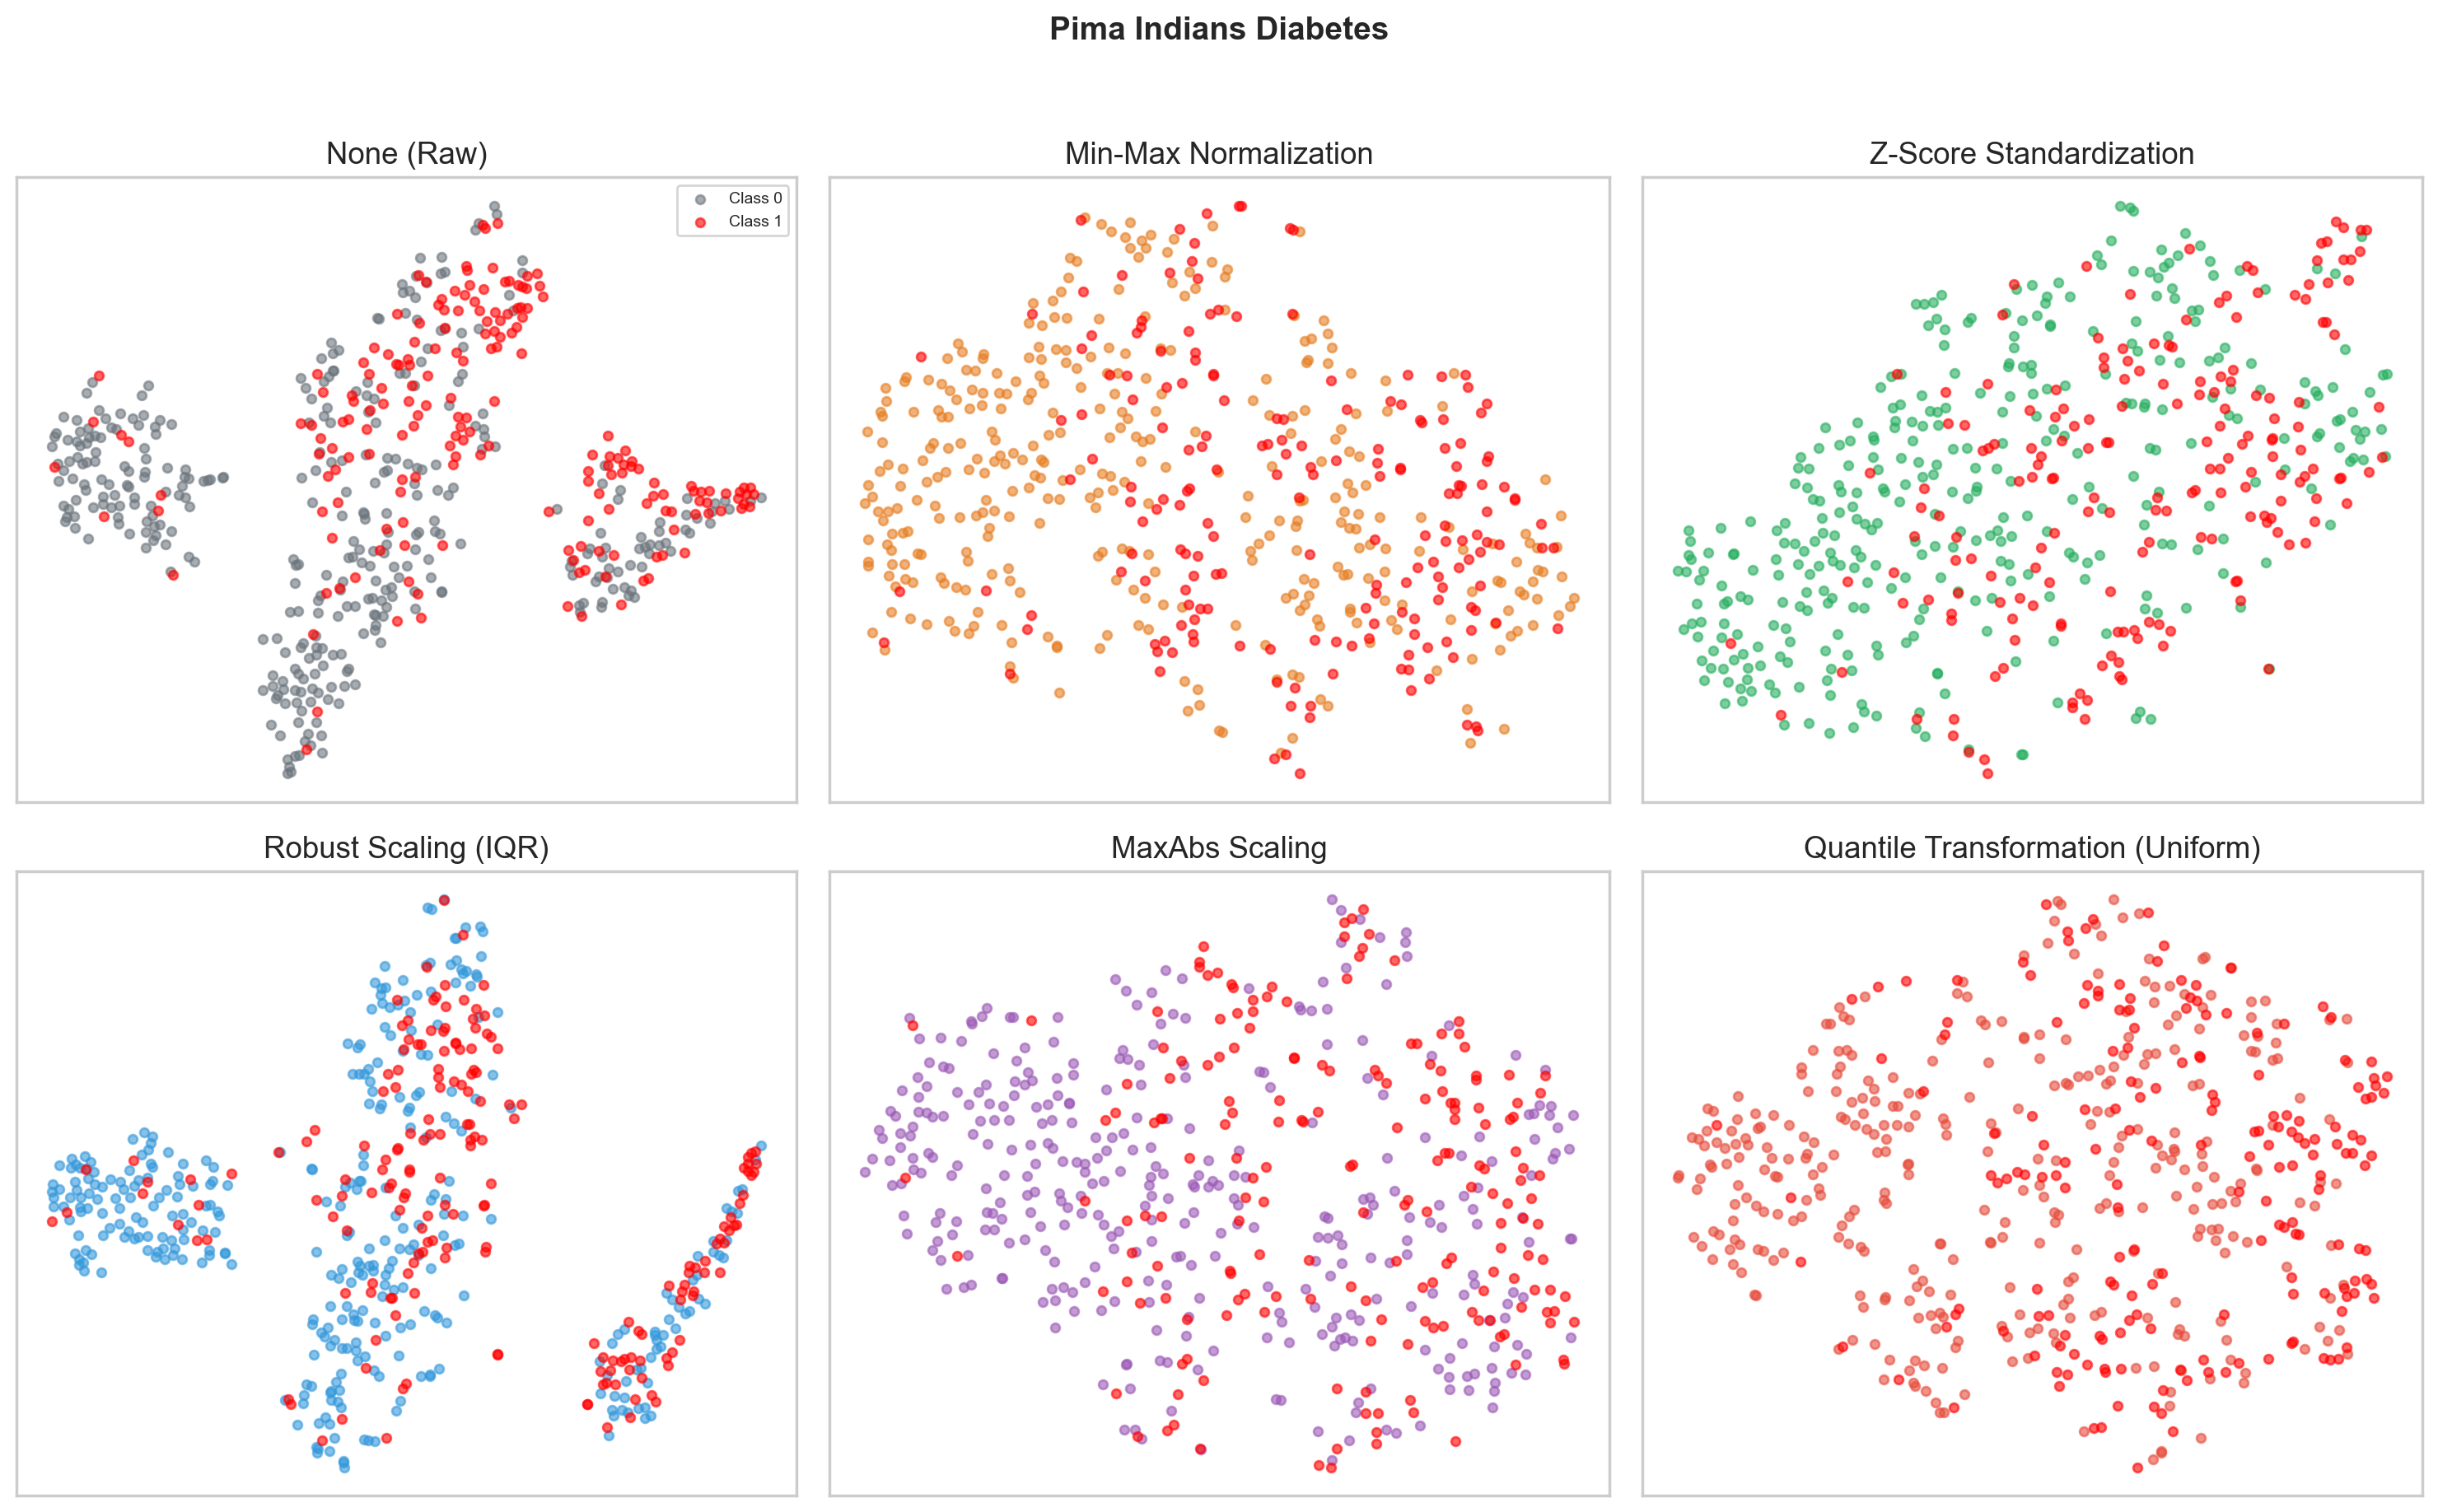
\includegraphics[width=0.85\textwidth]{figures/tsne_pima_diabetes.png}
\caption{Proyeksi \textit{t-SNE} Pima Indians Diabetes di bawah setiap teknik
penskalaan. Merah = diabetes, biru = sehat.}
\label{fig:tsne}
\end{figure}

\textbf{Pada data kimia dengan pengukuran terbatas (Wine), \textit{Z-Score}
juga unggul---bertentangan dengan intuisi umum bahwa \textit{Min-Max} optimal
untuk data terbatas.} Ketika dievaluasi sebagai permasalahan 3 kelas (vs.
binerisasi pada penelitian sebelumnya), \textit{Z-Score} mencapai 0,967
dibandingkan \textit{Min-Max} pada 0,954, mengindikasikan bahwa batas keputusan
multikelas memperoleh manfaat dari standardisasi yang mempertahankan jarak
relatif di seluruh pasangan kelas secara simultan.

\textbf{Pada data segmentasi citra (Segment), \textit{MaxAbs} mencapai skor
tertinggi (0,9455)}, sedikit mengungguli \textit{Min-Max} (0,9416). Ini adalah
satu-satunya \textit{dataset} di mana \textit{MaxAbs} memimpin, dan keunggulannya
kemungkinan berasal dari fitur tekstur yang memiliki rentang dinamis bervariasi
tanpa pencilan ekstrem.

\textbf{Pada data piksel yang telah berskala alami (Digits), penskalaan
memberikan manfaat minimal hingga negatif.} Data mentah (0,9732) dan
\textit{MaxAbs} (0,9728) secara virtual setara, sementara \textit{Robust
Scaling} justru menurunkan akurasi menjadi 0,9070.

\textbf{Pada data biologis multikelas (Yeast), semua \textit{scaler} bekerja
kurang memadai (0,54--0,58).} Yeast memiliki 10 kelas yang sangat tidak
seimbang dengan distribusi fitur yang tumpang tindih. \textit{Z-Score} memimpin
secara marginal (0,5765), namun akurasi absolut yang rendah mengindikasikan
bahwa penskalaan saja tidak dapat mengompensasi tumpang tindih kelas yang
inheren.

Jawaban untuk RQ3: \textbf{Karakteristik domain sangat menentukan \textit{scaler}
mana yang bekerja terbaik, dan pola ini berlaku pada pengaturan biner maupun
multikelas.} Hasil multikelas mencerminkan temuan biner untuk \textit{Z-Score},
mengonfirmasi bahwa keunggulannya bersifat generalisasi di luar kasus biner.

\subsection{Temuan Tambahan}
\label{sec:additional}

\textbf{Interaksi metrik jarak dengan penskalaan.} Untuk \textit{k-NN}, jarak
\textit{Manhattan} dengan \textit{scaler} yang sesuai mencapai hasil yang
sebanding dengan \textit{Euclidean}. Jarak \textit{Cosine} bekerja kompetitif
pada data berdimensi tinggi (Breast Cancer, Digits) namun menurun pada
\textit{dataset} dengan sampel kecil (Wine).

\textbf{\textit{Quantile Transformation} berada di bawah \textit{scaler}
linear.} Meskipun memiliki keunggulan teoretis dalam menangani distribusi
arbitrer, \textit{QuantileTransformer} menempati peringkat kelima secara
keseluruhan. Hal ini kemungkinan disebabkan oleh sensitivitas klasifikator
yang dievaluasi terhadap pemeliharaan jarak relatif, yang terdistorsi oleh
transformasi non-linear.

\textbf{\textit{MaxAbs Scaling} sebagai alternatif kokoh terhadap
\textit{Min-Max}.} Di seluruh \textit{dataset}, \textit{MaxAbs} berada di
tiga besar untuk 5 dari 6 \textit{dataset} dan tidak pernah menempati
peringkat terakhir. Rentang $[-1, 1]$-nya mempertahankan nilai nol dan pola
\textit{sparsity}, menjadikannya kandidat kuat untuk sistem produksi.

\textbf{\textit{Robust Scaling} dan \textit{Quantile} setara secara statistik}
($p = 0,596$), keduanya berada di bawah \textit{scaler} linear. Hal ini
mengindikasikan bahwa ketahanan terhadap pencilan saja tidak mencukupi---pemeliharaan
struktur jarak relatif lebih penting untuk klasifikator yang diuji.

% ============================================================
\section{Pembahasan}
\label{sec:discussion}

\subsection{Sintesis}
\label{sec:synthesis}

Ketiga pertanyaan penelitian, jika dipandang secara bersama-sama, memberikan
gambaran yang konsisten:

\textbf{Penskalaan selalu membantu, dan \textit{Z-Score} adalah \textit{default}
teraman---namun marginnya kecil.} Hasil agregat (\textit{Z-Score} $\approx$
\textit{Min-Max} $>$ \textit{MaxAbs} $>$ \textit{Robust} $\approx$
\textit{Quantile} $>$ Mentah) menyediakan titik awal, namun selisih sempit
berarti bahwa pertimbangan spesifik-domain, ukuran \textit{dataset}, dan
struktur multikelas seringkali lebih berpengaruh daripada peringkat global.

Dasar teoretis untuk interaksi ini jelas. Klasifikator berbasis jarak menghitung
besaran geometris yang terdistorsi oleh skala fitur yang tidak setara---metode
penskalaan linear apa pun yang menyetarakan rentang fitur dapat mengatasinya.
\textit{Z-Score} mempertahankan jarak relatif di bawah pencilan lebih baik
daripada \textit{Min-Max} karena tidak membatasi rentang hasil transformasi.
\textit{MaxAbs} menyediakan titik tengah dengan rentang $[-1, 1]$-nya yang
menghindari masalah pemampatan pencilan pada \textit{Min-Max}.

\subsection{Rekomendasi Praktis}
\label{sec:recommendations}

Berdasarkan sintesis di atas, kami mengusulkan kerangka keputusan berikut:

\textbf{Gunakan Standardisasi \textit{Z-Score} ketika:}
\begin{itemize}
  \item Data mengandung fitur dengan distribusi yang tidak diketahui atau
  campuran.
  \item \textit{Dataset} memiliki pencilan signifikan (medis, finansial, biologis).
  \item Permasalahan bersifat multikelas dengan batas kelas yang tumpang tindih.
  \item Diperlukan \textit{default} yang aman ketika pengetahuan domain tidak
  tersedia.
\end{itemize}

\textbf{Gunakan Normalisasi \textit{Min-Max} atau \textit{MaxAbs Scaling} ketika:}
\begin{itemize}
  \item Fitur memiliki batas alami yang diketahui (pembacaan sensor, pengukuran
  kimia).
  \item Mempertahankan \textit{sparsity} penting (\textit{MaxAbs} lebih disukai).
  \item \textit{Dataset} berdimensi tinggi dengan kelas seimbang.
\end{itemize}

\textbf{Gunakan \textit{Robust Scaling} atau \textit{Quantile Transformation} ketika:}
\begin{itemize}
  \item Terdapat pencilan ekstrem dan \textit{scaler} linear gagal.
  \item Catatan: ekspektasi kinerja setara dengan---tidak lebih baik dari---
  \textit{Z-Score}.
\end{itemize}

\textbf{Lewati penskalaan ketika:}
\begin{itemize}
  \item Fitur-fitur sudah berada dalam skala yang serupa (data piksel, survei
  \textit{Likert}).
  \item Klasifikator berbasis pohon (peningkatan dapat diabaikan).
  \item Diperlukan perbandingan \textit{baseline}.
\end{itemize}

\subsection{Perbandingan dengan Penelitian Terdahulu}
\label{sec:comparison}

Temuan kami sejalan dengan dan memperluas studi komparatif sebelumnya, khususnya
de Amorim dkk. \cite{amorim2023scaling} dan Demircioglu
\cite{demircioglu2024normalization}. Henderi dkk.~\cite{henderi2021minmax}
menemukan \textit{Min-Max} lebih unggul pada klasifikasi kanker payudara dengan
\textit{k-NN}---kami mengonfirmasi hal ini untuk \textit{k-NN} namun menunjukkan
bahwa \textit{Z-Score} melampaui \textit{Min-Max} ketika klasifikatornya adalah
SVM dan ketika evaluasi mencakup data multikelas. Pinheiro
dkk.~\cite{pinheiro2025scaling} menunjukkan bahwa metode ensemble kokoh terhadap
penskalaan sementara SVM sangat sensitif; hasil kami mendukung temuan ini dan
memperluasnya ke \textit{MaxAbs Scaling}, yang bekerja kompetitif dengan
\textit{Z-Score} pada sebagian besar kombinasi klasifikator--\textit{dataset}.

Sertifikasi \textit{MaxAbs Scaling} dan \textit{Quantile Transformation}---yang
tidak ada dalam sebagian besar perbandingan sebelumnya
\cite{pagan2023scaling,henderi2021minmax,firmansyah2024stroke,pristyanto2022diabetes}---mengungkapkan
 bahwa \textit{MaxAbs} merupakan alternatif yang viable terhadap
\textit{Min-Max}, khususnya pada data berdimensi tinggi.

\subsection{Keterbatasan}
\label{sec:limitations}

\begin{itemize}
  \item \textbf{Hiperparameter bawaan:} Tidak dilakukan penalaan hiperparameter
  di luar rentang $k$ pada \textit{k-NN}. Klasifikator yang dioptimalkan mungkin
  merespons penskalaan secara berbeda.
  \item \textbf{Cakupan \textit{dataset}:} Enam \textit{dataset} di empat domain
  memberikan keragaman yang memadai namun \textit{dataset} tambahan akan
  memperkuat generalisabilitas.
  \item \textbf{Cakupan klasifikator:} \textit{Deep learning}, \textit{naive
  Bayes}, dan metode \textit{gradient boosting} tidak dievaluasi.
  \item \textbf{Interaksi fitur:} Kami tidak meneliti interaksi antara penskalaan
  dan seleksi fitur atau reduksi dimensionalitas.
\end{itemize}

\subsection{Penelitian Selanjutnya}
\label{sec:future}

Ekstensi yang mungkin meliputi:
\begin{itemize}
  \item Perluasan ke \textit{dataset} berdimensi tinggi (teks, genomika) dengan
  ribuan fitur.
  \item Penelitian interaksi dengan optimalisasi hiperparameter.
  \item Evaluasi pada arsitektur \textit{deep learning} di mana penskalaan
  berinteraksi dengan fungsi aktivasi.
  \item Pengembangan sistem rekomendasi \textit{scaler} otomatis berdasarkan
  meta-fitur \textit{dataset}.
\end{itemize}

% ============================================================
\section{Kesimpulan}
\label{sec:conclusion}

Studi ini mengevaluasi 3.384 konfigurasi klasifikator dengan validasi silang
bertingkat 5-lipat (16.920 total pemasangan) yang membandingkan enam teknik
penskalaan pada tujuh klasifikator dan enam \textit{dataset} (termasuk empat
\textit{dataset} multikelas). Ketiga pertanyaan penelitian dijawab sebagai
berikut:

\textbf{RQ1 (peringkat keseluruhan):} Standardisasi \textit{Z-Score} menempati
peringkat pertama (0,8561), setara secara statistik dengan \textit{Min-Max}
(0,8530, $p=0,123$) namun secara signifikan di depan \textit{MaxAbs} (0,8506,
$p=0,002$). Semua \textit{scaler} secara signifikan mengungguli data mentah
($p<0,01$).

\textbf{RQ2 (ketergantungan klasifikator):} SVM (RBF) adalah yang paling sensitif
terhadap penskalaan (+7,7\% peningkatan), \textit{k-NN} menunjukkan sensitivitas
sedang (+4,6--6,0\%), dan model berbasis pohon hampir invarian ($<$0,2\%).

\textbf{RQ3 (ketergantungan domain):} \textit{Z-Score} unggul pada data medis dan
data biologis multikelas. \textit{MaxAbs} unggul pada data berdimensi tinggi
yang seimbang. Data mentah memadai ketika fitur telah berskala alami. Hasil
multikelas mengonfirmasi bahwa keunggulan \textit{Z-Score} bersifat generalisasi
di luar klasifikasi biner.

Temuan tambahan meliputi: (i) \textit{MaxAbs Scaling} merupakan alternatif kuat
terhadap \textit{Min-Max}; (ii) \textit{Quantile Transformation} berada di bawah
\textit{scaler} linear, mengindikasikan bahwa pemeliharaan jarak lebih penting
daripada normalisasi distribusi; dan (iii) selisih antar teknik penskalaan kecil
($<$0,8\% antara tiga teratas), menekankan bahwa pertimbangan spesifik-domain
harus memandu pemilihan akhir.

Hasil ini menunjukkan bahwa pertanyaan ``\textit{scaler} mana yang terbaik?''
tidak lengkap---pertanyaan praktisnya adalah ``\textit{scaler} mana yang terbaik
untuk \emph{klasifikator saya}, \emph{data saya}, dan \emph{tipe permasalahan
saya}?'' Kerangka keputusan pada Bagian~\ref{sec:recommendations} menyediakan
jawaban praktis.

% ============================================================
\bibliography{references}
\label{sec:references}

\end{document}
